\documentclass{book}
\usepackage{amsmath, amssymb} % Pour les mathématiques
\usepackage{graphicx} % Pour inclure des images
\usepackage{hyperref} % Pour les liens, si nécessaire

\begin{document}

% Partie préliminaire : Table des matières
\frontmatter
\title{Neophysique}
\author{Henri}
\date{\today}
\maketitle
\tableofcontents % Génération automatique de la table des matières

% Partie principale : Chapitres
\mainmatter
\chapter{Chapitre 1 : Introduction à la néophysique}
\input{neophi.tex} % Intègre le contenu du fichier "neophi.tex"

\chapter{Chapitre 2 : Concepts avancés}
\input{neoa.tex} % Intègre le contenu du fichier "neoa.tex"

\chapter{Chapitre 3 : Illustrations}
Voici deux images importantes pour la néophysique :

\begin{figure}[h]
    \centering
    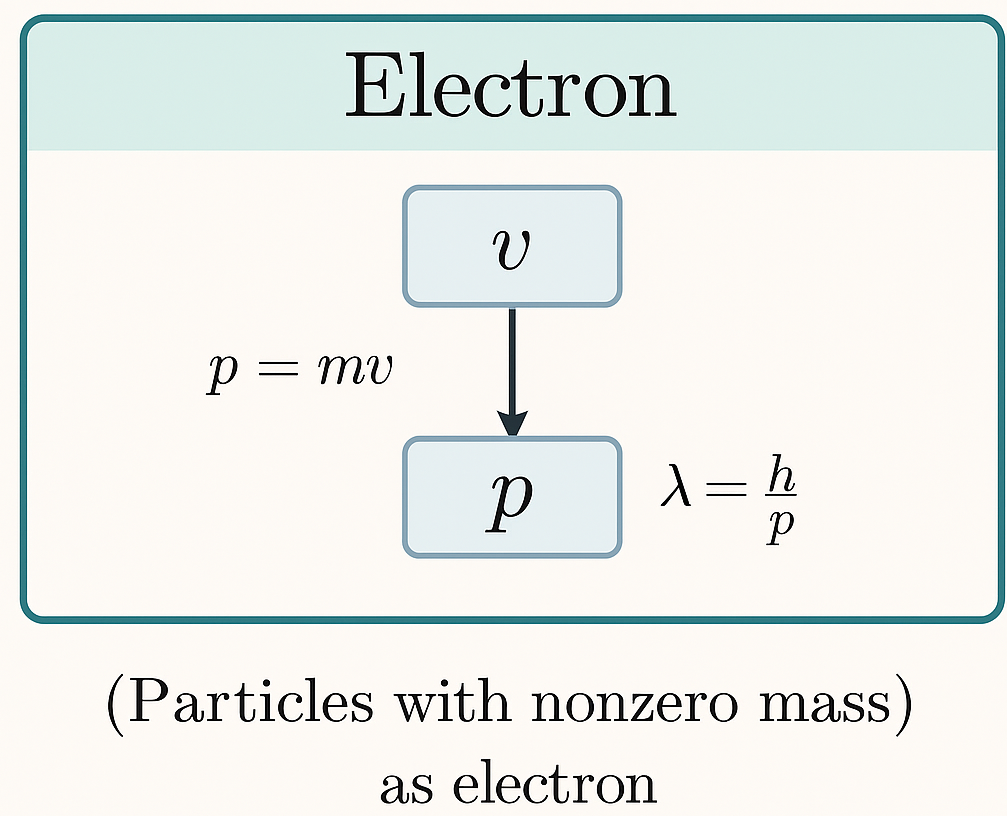
\includegraphics[width=0.7\textwidth]{electron.png} % Image "electron.png"
    \caption{Diagramme de l'électron}
    \label{fig:electron}
\end{figure}

\begin{figure}[h]
    \centering
    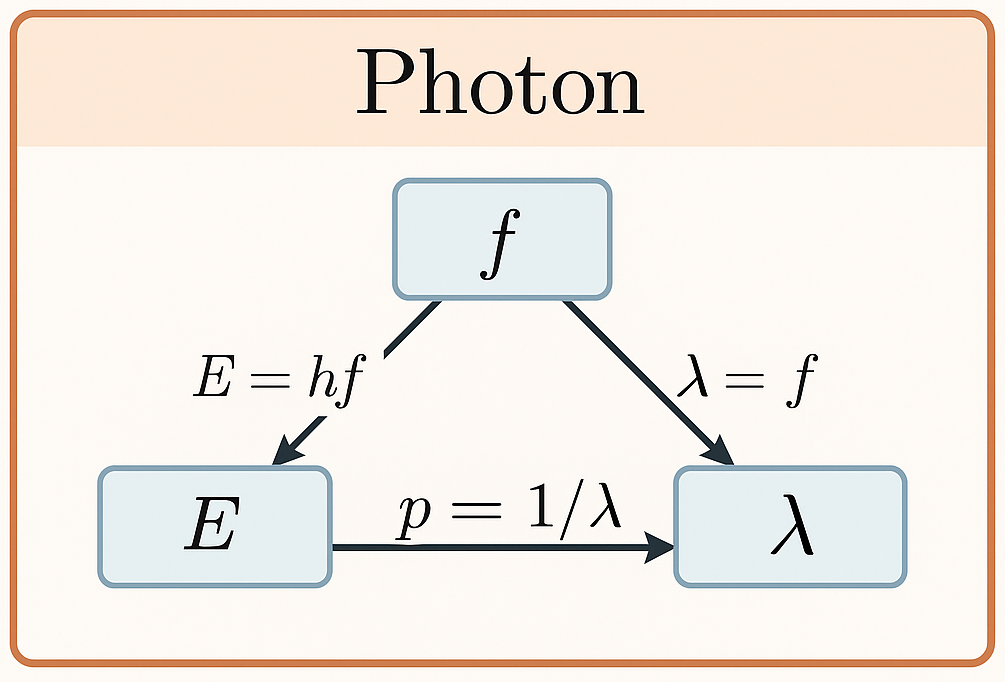
\includegraphics[width=0.7\textwidth]{photon.png} % Image "photon.png"
    \caption{Diagramme du photon}
    \label{fig:photon}
\end{figure}

\end{document}

